\section{Results}
\label{sec:results}

The results are organised by analysis and linked to the contributions introduced in Section~\ref{sec:introduction}. Primary ensemble discrimination and transfer to unseen sites are reported first, together with comparison to published ABIDE-I studies. The remaining analyses then examine cognitive ability, motion-matched functional-system differences, feature-selection scope, classifier family, symptom-severity associations, covariance shrinkage in the windowed representation, probability calibration, and attribution of model scores to functional-system pairs. The feature-selection analysis is treated as a methodological check rather than as one of the five main contributions. Secondary findings are reported afterwards, including relevant null results and limitations. Throughout, AUROC and accuracy are identified as either participant-pooled estimates or fold means, following Section~\ref{subsubsec:performance-measures}, because these summaries answer different aggregation questions.

\subsection{Classification performance and transfer to unseen sites}
\label{subsec:results-performance}

The highest AUROC of the connectivity-only configurations is obtained with the primary
ensemble under both validation protocols (Table~\ref{tab:configurations}). Specifically, a
fold-mean AUROC of 0.775 is obtained under pooled ten-fold validation, and a fold-mean
AUROC of 0.773 is obtained under LOSO validation. However, the gain over the
best single representation, the windowed tangent mean, is small ($+0.009$ in
participant-pooled AUROC).
Moreover, this gain is not distinguished from chance (unadjusted DeLong $p=0.066$), so it
is not presented as an established improvement. The rank-mean ensemble
(Section~\ref{subsubsec:rank-fusion}) is, in turn, reported for comparison only. Because its score is
not a probability, it has no 0.5 decision threshold, and no accuracy is reported for it.

\begin{table}[pos=htb]
\centering
\caption{Discrimination is evaluated for the ensemble and its individual members in the primary cohort of 871 participants. AUROC and accuracy are reported as fold means, with SD calculated across the outer folds. Because no probability scale is defined for the rank-mean ensemble, accuracy is not reported for this model.}
\label{tab:configurations}
\small
\begin{tabular}{@{}lcccccc@{}}
\toprule
 & \multicolumn{3}{c}{Pooled ten-fold} & \multicolumn{3}{c}{LOSO} \\
\cmidrule(lr){2-4}\cmidrule(l){5-7}
Configuration & AUROC & SD & Accuracy & AUROC & SD & Accuracy \\
\midrule
Ensemble, probability mean (adopted) & 0.775 & 0.040 & 0.707 & 0.773 & 0.087 & 0.684 \\
Windowed tangent, mean & 0.767 & 0.044 & 0.695 & 0.771 & 0.082 & 0.670 \\
Ensemble, rank mean & 0.756 & 0.038 & -- & 0.750 & 0.091 & -- \\
Static tangent & 0.756 & 0.048 & 0.692 & 0.757 & 0.104 & 0.643 \\
Correlation & 0.750 & 0.040 & 0.683 & 0.743 & 0.083 & 0.655 \\
\bottomrule
\end{tabular}
\end{table}

Participant-pooled estimates show similar discrimination under pooled ten-fold and LOSO validation (Table~\ref{tab:performance}; Figure~\ref{fig:performance}a). AUROC is 0.776 under pooled ten-fold validation, with a 95\% DeLong interval of 0.745--0.807, and 0.774 under LOSO validation, with an interval of 0.744--0.805. Under pooled validation, sensitivity and specificity are similar at 0.705 and 0.709, whereas under LOSO validation sensitivity is higher than specificity at 0.742 and 0.684. Site-clustered bootstrap intervals are wider than the parametric intervals. For pooled validation, the AUROC interval widens to 0.733--0.807 and the accuracy interval to 0.670--0.737, compared with 0.745--0.807 and 0.676--0.736 from DeLong and Wilson intervals. Under LOSO validation, the AUROC interval widens to 0.726--0.808 and the accuracy interval to 0.661--0.748, compared with 0.744--0.805 and 0.680--0.740. The larger change occurs mainly at the lower bounds, but all AUROC intervals remain above 0.5. The choice of penalty strength is also stable to the scope of nesting. When the tangent reference and feature scaler are refitted within every inner split (Section~\ref{subsubsec:nested-penalty}), the selected value changes in only 2 of 30 member fits under pooled validation and 2 of 60 under LOSO validation, with inner-AUROC differences no larger than 0.0004. Participant-pooled AUROC changes from 0.7760 to 0.7756 and from 0.7745 to 0.7746, while accuracy changes from 0.707 to 0.706 and from 0.711 to 0.705. Extending the penalty grid down to $10^{-5}$ still selects 0.001 in 81 of 90 member fits, with AUROCs of 0.7743 and 0.7747. Finally, cohort counts are consistent with the released records. Of 1,112 ABIDE-I phenotypic records, 1,035 have a preprocessed derivative, and 871 meet the three-rater primary rule with usable regional time series, comprising 403 autistic and 468 non-autistic participants. The wider QC cohort is defined by an acceptable functional-image rating from the third rater and contains 1,035 records, of which 1,032 have regional time series. The two 1,035-record sets overlap in 1,033 participants.

\begin{table}[t]
\centering
\caption{Participant-pooled performance of the primary ensemble in the primary cohort
(871 participants), with 95\% intervals. AUROC carries DeLong intervals; accuracy,
sensitivity and specificity carry Wilson intervals.}
\label{tab:performance}
\small
\begin{tabular}{@{}lcccc@{}}
\toprule
Validation & AUROC & Accuracy & Sensitivity & Specificity \\
\midrule
Pooled ten-fold & 0.776 (0.745--0.807) & 0.707 (0.676--0.736) & 0.705 (0.658--0.747) & 0.709 (0.667--0.749) \\
LOSO & 0.774 (0.744--0.805) & 0.711 (0.680--0.740) & 0.742 (0.697--0.782) & 0.684 (0.640--0.724) \\
\bottomrule
\end{tabular}
\end{table}

\begin{figure}[pos=tbp]
\centering
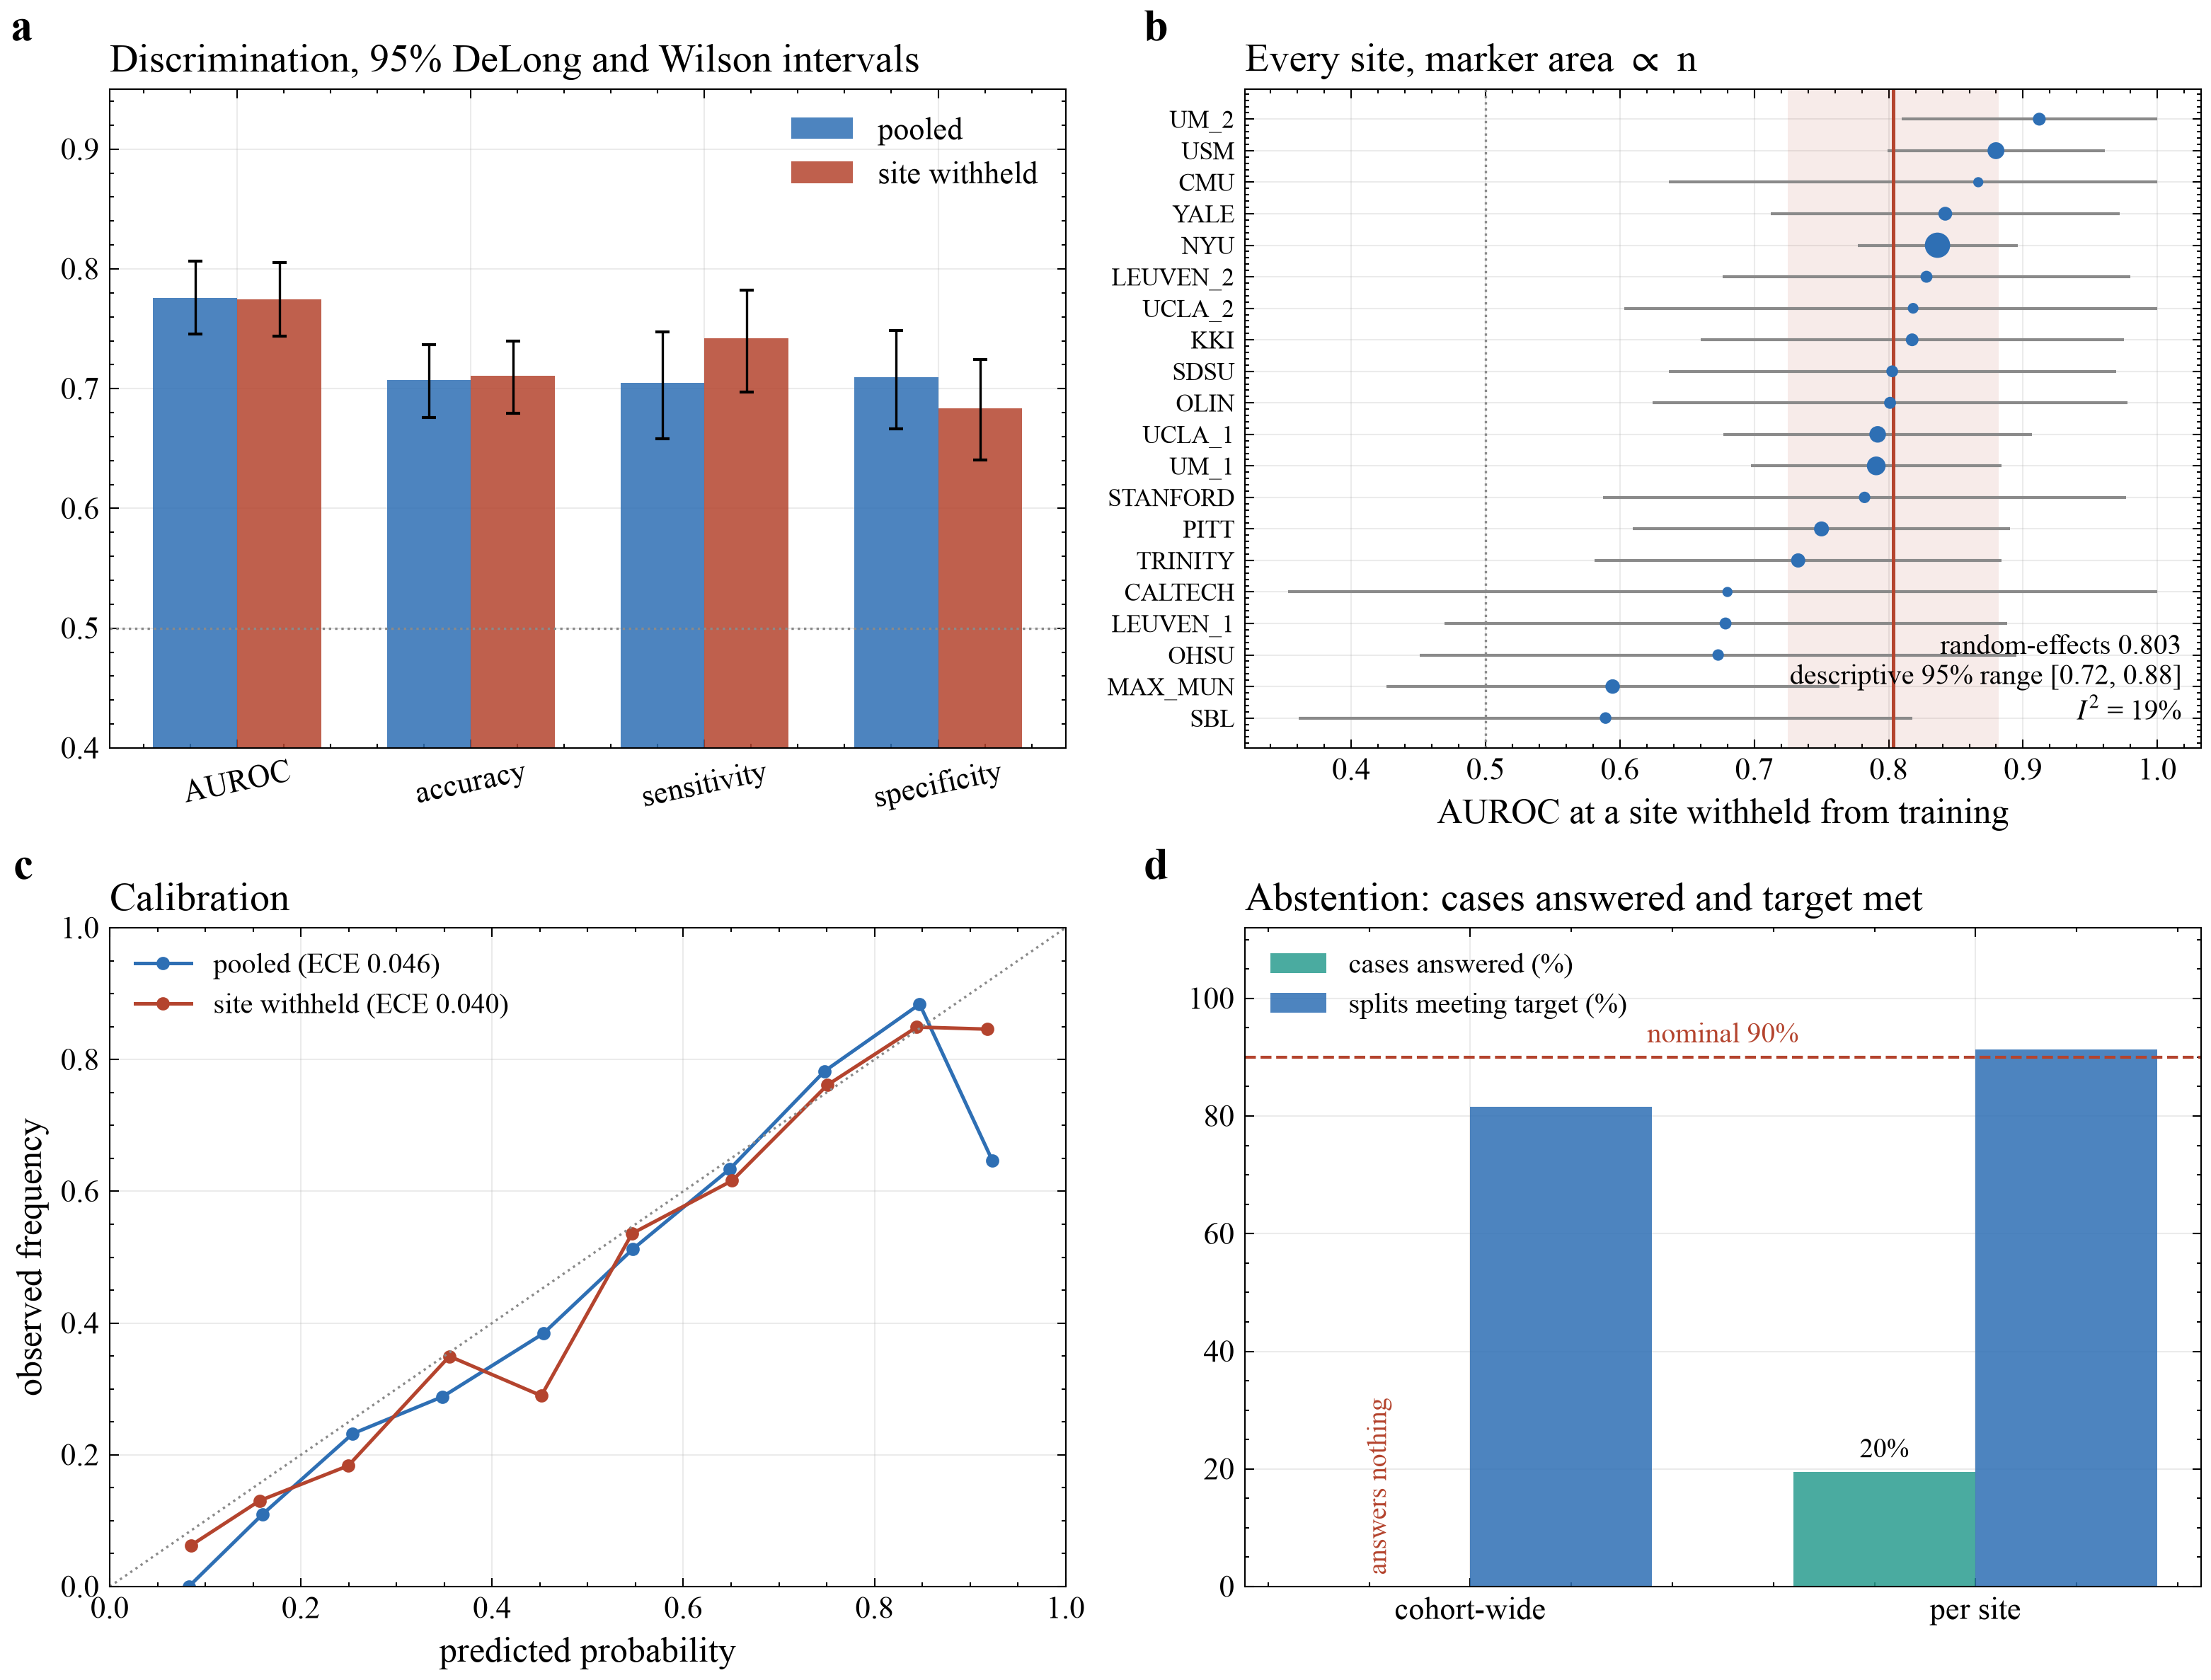
\includegraphics[width=\linewidth]{fig_performance}
\caption{Discrimination, per-site transfer, calibration, and abstention of the primary ensemble. (a) Discrimination under both validation protocols, with 95\% DeLong and Wilson intervals reported as lower-bound estimates of uncertainty. (b) AUROC for each site when that site is withheld from training, with marker area proportional to the number of participants. The random-effects mean and the descriptive interval from Equation~\eqref{eq:prediction-interval} are shown; this interval describes the observed sites and is not interpreted as a prediction for an unseen site. (c) Native predicted probabilities against observed frequencies in ten equal-width bins. (d) Cohort-wide and per-site abstention under LOSO validation, showing the percentage of participants answered when the threshold is set on the full sample and the percentage of held-out half-splits in which the error target is achieved, relative to the nominal 90\%.}
\label{fig:performance}
\end{figure}

Variation across sites is summarised with a random-effects model as a descriptive sensitivity analysis. Combining the 20 site-specific estimates gives a random-effects mean AUROC of 0.803 (Figure~\ref{fig:performance}b). Between-site heterogeneity is modest and not statistically distinguishable from chance ($Q=23.5$ on 19 degrees of freedom, $p=0.22$; $I^2=19\%$). The descriptive 95\% interval from Equation~\eqref{eq:prediction-interval} spans 0.725--0.882. Because LOSO estimates share training data, this interval is not treated as a validated prediction interval for an independent site. Site-level AUROC ranges from 0.589 at SBL to 0.912 at UM\_2. Two sites, SBL and MAX\_MUN, fall below 0.65, and the 95\% intervals of five sites (CALTECH, LEUVEN\_1, MAX\_MUN, OHSU, and SBL) include 0.5. These wide intervals are expected because the median site contains only about 30 participants. Phenotypic variables provide some additional discrimination but contribute little beyond connectivity. The phenotype model reaches an AUROC of about 0.62 on its own (Section~\ref{par:phenotype-model}), and adding it to the ensemble increases participant-pooled AUROC by about 0.004 (unadjusted $p=0.041$; $q=0.11$, reported for reference only). The phenotype member is therefore not retained. For comparison with published ABIDE-I studies, the wider QC cohort is used because its QC definition yields 1,035 eligible participants, matching the published count. Three participants lack usable time series, leaving 1,032 for analysis. In this cohort, pooled ten-fold validation gives a participant-pooled accuracy of 0.706 (95\% Wilson interval 0.678--0.733). Published accuracies of 0.700, 0.703, and 0.708 are reported by \citet{Heinsfeldetal2018}, \citet{Eslamietal2019}, and \citet{AlmuqhimSaeed2021}, respectively; these values are cited as reported and are not recomputed here.

\begin{table}[t]
\centering
\caption{Placement against published work on ABIDE-I resting-state functional
connectivity. Values for the other studies are as reported by their authors; n.r., not
reported. For the ensemble rows, AUROC is participant-pooled and accuracy is the fold mean,
which agrees with the participant-pooled value to three decimals. For the tangent-model
row, AUROC and accuracy are fold means. The unseen-site column gives the
LOSO AUROC, with its difference from the pooled ten-fold value in brackets.}
\label{tab:published-comparison}
\small
\setlength{\tabcolsep}{4pt}
\begin{tabular}{@{}>{\raggedright\arraybackslash}p{0.24\linewidth}cccccc@{}}
\toprule
Study & Accuracy & AUROC & Sample & Procedure & AUROC, unseen site & ECE \\
\midrule
\citet{Heinsfeldetal2018} & 0.700 & n.r. & 1,035 & 10-fold & n.r. & n.r. \\
\citet{Eslamietal2019} & 0.703 & n.r. & 1,035 & 10-fold & n.r. & n.r. \\
\citet{AlmuqhimSaeed2021} & 0.708 & n.r. & 1,035 & 10-fold & n.r. & n.r. \\
This work, ensemble & 0.707 & 0.776 & 871 & nested 10-fold & 0.774 ($-0.002$) & 0.046 \\
This work, ensemble, wider QC cohort & 0.706 & 0.789 & 1,032 & nested 10-fold & 0.783 ($-0.006$) & 0.023 \\
This work, tangent model, wider QC cohort & 0.696 & 0.766 & 1,032 & nested 10-fold & -- & -- \\
\bottomrule
\end{tabular}
\end{table}

The published accuracy values in Table~\ref{tab:published-comparison} are too close to support a clear separation between methods, particularly because the comparison studies do not report confidence intervals. With these sample sizes, the expected uncertainty is roughly $\pm0.03$, whereas the three published accuracies differ by only 0.008. Two additional measures are therefore reported for the present study without direct comparison to the published results. AUROC is 0.776 under pooled validation and 0.774 under LOSO validation, while the ECE is 0.046 (Section~\ref{subsec:results-calibration}). The present accuracy is also obtained without fitting outcome-dependent steps before the data split. This distinction is important because global label-informed feature selection produces a markedly higher performance estimate in Section~\ref{subsec:results-selection-scope}. Performance also varies with cohort definition. The static tangent model reaches a fold-mean AUROC of 0.756 in the primary cohort of 871 participants and 0.766 in the wider cohort of 1,032 participants. Because many participants excluded by the primary definition have greater head motion or preprocessing problems, and these exclusions are not balanced across diagnostic groups, the difference between cohorts may partly reflect data quality and cohort composition rather than connectivity alone.

\subsection{Cognitive ability and detection}
\label{subsec:results-cognitive-ability}

Discrimination is lower in the higher-IQ autistic subgroups in the unmatched band analysis, contributing to the fourth study contribution. Because these subgroup analyses are exploratory (Sections~\ref{par:cognitive-sex-subgroups} and~\ref{subsubsec:analysis-status}), the pattern is interpreted descriptively. To keep the comparison group constant, all 468 non-autistic participants are used as the reference for every IQ band, while only autistic participants are divided by full-scale IQ. Under pooled ten-fold validation, AUROC decreases from 0.873 for autistic participants with full-scale IQ below 85 to 0.719 for those with IQ 115 or above (Table~\ref{tab:iq-bands}; Figure~\ref{fig:group-differences}d). A similar pattern is observed under LOSO validation, where AUROC decreases from 0.871 to 0.709. However, the autistic IQ bands still differ from the fixed non-autistic reference group in full-scale IQ, so this unmatched comparison does not isolate IQ from group composition. The matched analysis below addresses this remaining difference.

\begin{table}[t]
\centering
\caption{AUROC by full-scale IQ band of the autistic participants, each band scored
against the same comparison group of all 468 non-autistic participants.}
\label{tab:iq-bands}
\small
\begin{tabular}{@{}lccc@{}}
\toprule
Autistic participants & $n$ & Pooled ten-fold & LOSO \\
\midrule
Full-scale IQ below 85 & 40 & 0.873 & 0.871 \\
Full-scale IQ 85--99 & 97 & 0.815 & 0.816 \\
Full-scale IQ 100--114 & 126 & 0.781 & 0.788 \\
Full-scale IQ 115 or above & 113 & 0.719 & 0.709 \\
\bottomrule
\end{tabular}
\end{table}

\begin{figure}[pos=tbp]
\centering
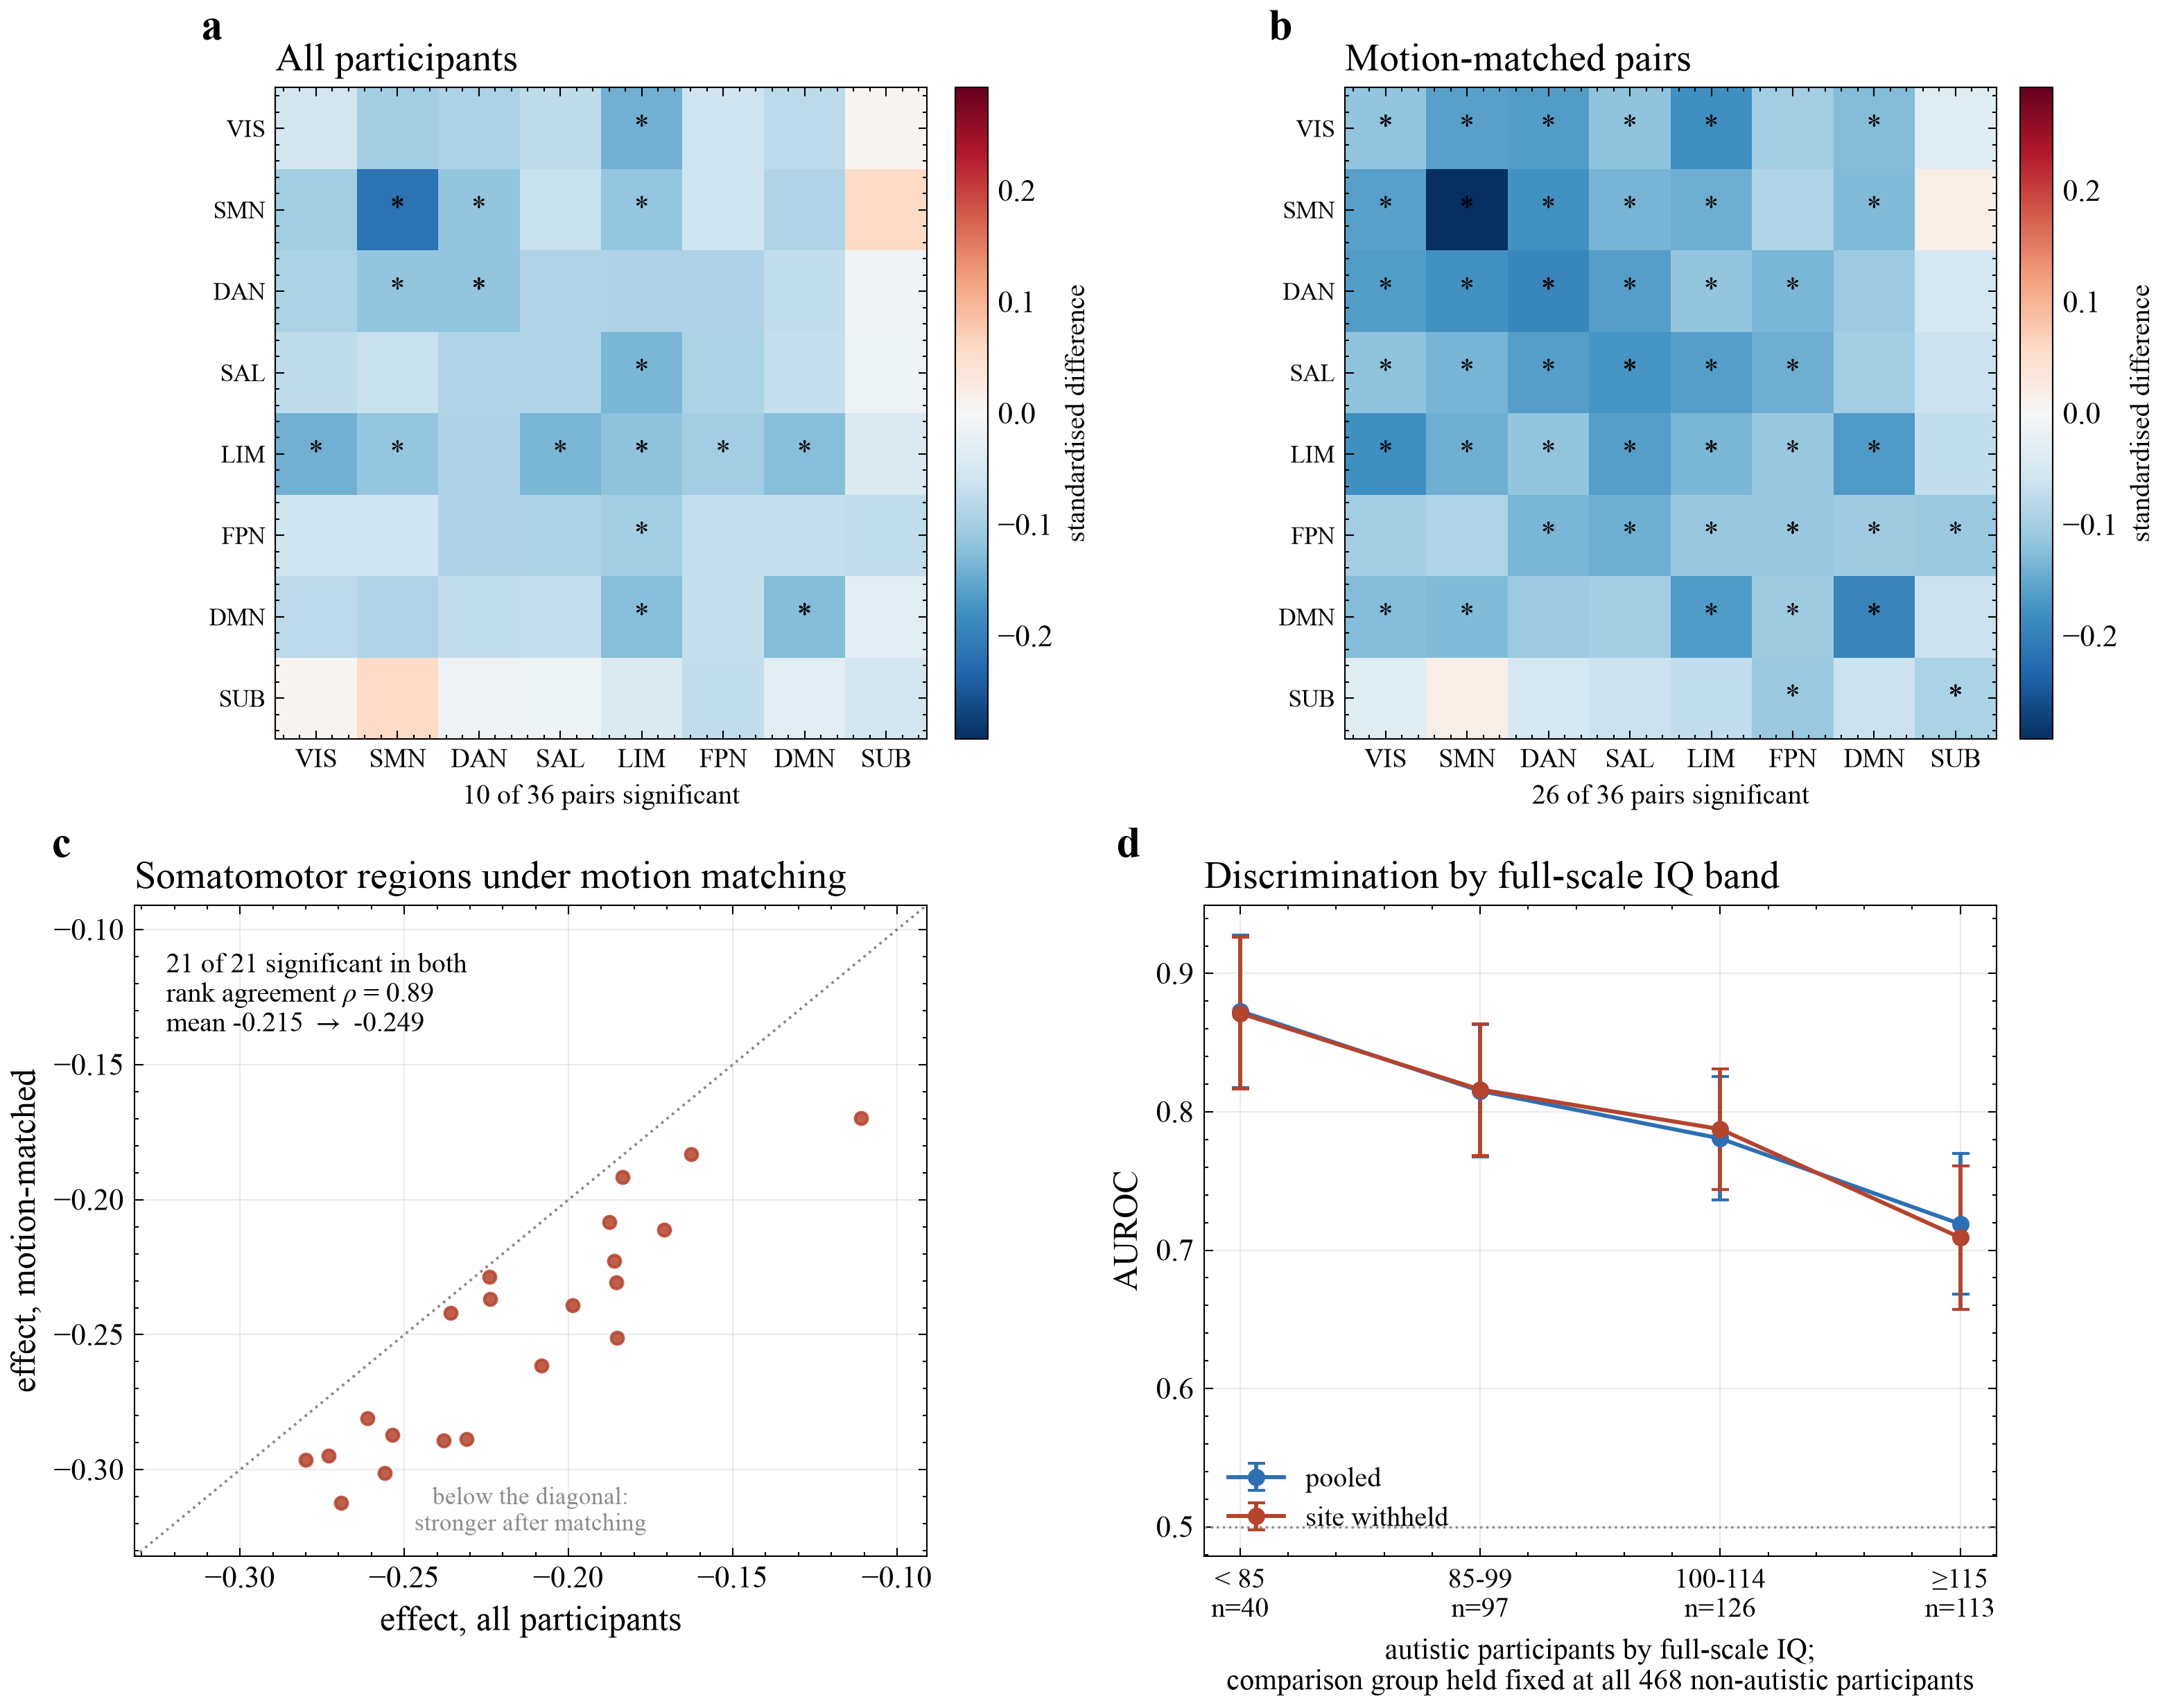
\includegraphics[width=\linewidth]{fig_groupdiff}
\caption{Group differences in functional-system connectivity and the effect of motion
matching. (a, b) Standardised difference for every pair of systems (system codes as in Figure~\ref{fig:overview}) in all participants and
in within-site pairs matched for head motion, on a shared colour scale; asterisks mark
pairs with BH-FDR $q<0.05$. (c) The effect of each somatomotor region in all
participants plotted against its effect in motion-matched pairs; points below the diagonal
are stronger once motion is matched. (d) Discrimination by full-scale IQ band among
autistic participants (below 85, 85--99, 100--114, and 115 or above), each against all 468
non-autistic participants, under both validation protocols.}
\label{fig:group-differences}
\end{figure}

The same pattern is observed when both groups are divided into quartiles of site-centred full-scale IQ (Table~\ref{tab:iq-quartiles}). Under pooled ten-fold validation, AUROC decreases from 0.833 in the lowest quartile to 0.709 in the highest. Because autistic participants have lower full-scale IQ overall (Table~\ref{tab:participants}), this stratified comparison may still reflect differences in IQ between the groups. To reduce this imbalance, autistic participants are matched to non-autistic participants from the same site within five full-scale IQ points. This produces 274 matched pairs under pooled ten-fold validation and 275 pairs under LOSO validation.

\begin{table}[t]
\centering
\caption{AUROC by quartile of site-centred full-scale IQ, in all participants and in
participants matched on full-scale IQ within site. The matched counts are given for pooled
ten-fold and LOSO validation, respectively.}
\label{tab:iq-quartiles}
\small
\begin{tabular}{@{}lcccccc@{}}
\toprule
 & \multicolumn{3}{c}{All participants} & \multicolumn{3}{c}{IQ-matched participants} \\
\cmidrule(lr){2-4}\cmidrule(l){5-7}
Quartile & $n$ & Pooled ten-fold & LOSO & $n$ (pooled / LOSO) & Pooled ten-fold & LOSO \\
\midrule
Q1 & 204 & 0.833 & 0.825 & 137 / 144 & 0.855 & 0.848 \\
Q2 & 203 & 0.794 & 0.793 & 137 / 132 & 0.700 & 0.735 \\
Q3 & 201 & 0.746 & 0.745 & 138 / 137 & 0.751 & 0.737 \\
Q4 & 203 & 0.709 & 0.705 & 136 / 137 & 0.756 & 0.756 \\
\bottomrule
\end{tabular}
\end{table}

After IQ matching, discrimination remains highest in the lowest quartile but no longer declines consistently across the upper three. Under pooled ten-fold validation, AUROC is 0.855 in the lowest quartile and ranges from 0.700 to 0.756 in the remaining quartiles; under LOSO validation, the corresponding values are 0.848 and 0.735--0.756. This suggests that part of the original IQ gradient reflects between-group differences in IQ. Complementary within-group analyses show a negative association between classifier score and cognitive ability among autistic participants, but not among non-autistic participants. After adjustment for site, age, and mean FD, the pooled ten-fold score correlates with full-scale IQ at $\rho=-0.180$ ($p=0.0004$, $n=376$) in autistic participants, compared with $\rho=+0.048$ ($p=0.3208$, $n=435$) in non-autistic participants. Similar patterns are observed for verbal and performance IQ and under both validation protocols. Diagnosis-by-IQ interaction models further test this difference directly while adjusting for age, sex, mean FD, and site. The interaction remains significant after BH-FDR correction for full-scale IQ ($\beta=-0.176$, $q=0.025$) and verbal IQ ($\beta=-0.205$, $q=0.025$) under pooled ten-fold validation, and for both measures under LOSO validation ($q=0.033$). The interaction for performance IQ does not survive correction ($q=0.082$). These results indicate that the negative association between classifier score and cognitive ability is stronger in autistic participants for full-scale and verbal IQ.

\begin{table}[t]
\centering
\caption{Spearman correlation between classifier score and IQ within each diagnostic group, reported as $\rho$ ($p$). Before correlation, both variables are residualised for site, age, and mean FD. The p-values are not adjusted for multiple comparisons.}
\label{tab:iq-correlations}
\small
\setlength{\tabcolsep}{4pt}
\begin{tabular}{@{}lccccc@{}}
\toprule
 & & \multicolumn{2}{c}{Autistic} & \multicolumn{2}{c}{Non-autistic} \\
\cmidrule(lr){3-4}\cmidrule(l){5-6}
Measure & $n$ (autistic / non-autistic) & Pooled ten-fold & LOSO & Pooled ten-fold & LOSO \\
\midrule
Full-scale IQ & 376 / 435 & $-0.180$ (0.0004) & $-0.179$ (0.0005) & $+0.048$ (0.3208) & $+0.022$ (0.6466) \\
Verbal IQ & 342 / 379 & $-0.182$ (0.0007) & $-0.189$ (0.0004) & $+0.039$ (0.4547) & $+0.001$ (0.9892) \\
Performance IQ & 344 / 391 & $-0.152$ (0.0047) & $-0.147$ (0.0062) & $+0.007$ (0.8862) & $-0.005$ (0.9271) \\
\bottomrule
\end{tabular}
\end{table}

The absence of a comparable score--IQ association in non-autistic participants argues against a general relation between cognitive ability and classifier score. This interpretation is strengthened by the diagnosis-by-IQ interaction results, which remain significant for full-scale and verbal IQ, although full-scale IQ varies less among non-autistic participants (Table~\ref{tab:participants}). The association is also consistent with the verbal-IQ dependence reported in ABIDE by \citet{Nielsenetal2013}. However, the IQ-matched upper quartiles do not show a monotonic decline in AUROC, so the exploratory analyses do not establish a simple IQ-specific gradient in detectability. Instead, they indicate that measured ABIDE-I performance varies with the cognitive composition of the autistic sample, such that the same method can yield different AUROC values in cohorts with different IQ distributions. No corresponding reduction in discrimination is observed among female participants. Under pooled ten-fold validation, AUROC is 0.827 (0.760--0.895, $n=144$) in female participants and 0.764 (0.730--0.798, $n=727$) in male participants; under LOSO validation, the corresponding values are 0.806 (0.735--0.878) and 0.767 (0.733--0.801). Because these intervals overlap and the female subgroup is small, no sex difference in discrimination is inferred.

\subsection{Functional-system differences under motion matching}
\label{subsec:results-system-differences}

Functional-system differences are examined as exploratory group contrasts, and the motion-matched somatomotor result contributes to the third study contribution. To reduce the 19,110 connection-level effects to a more interpretable scale, regions are grouped into the seven cortical systems of \citet{Yeoetal2011} plus a subcortical/cerebellar class, producing 36 system pairs with 21--1,462 connections each (median 441). Connection values are adjusted for acquisition site, mean framewise displacement, age, and sex before system-level effects are calculated, and significance is assessed by permuting diagnostic labels within site. In the 863-participant group-contrast cohort, 10 of 36 system pairs remain significant after correction, and all show lower connectivity in autistic participants (Table~\ref{tab:system-pairs}; Figure~\ref{fig:group-differences}a). Overall, 34 of 36 system-pair effects are negative, with no significant increases. The largest reduction occurs within the somatomotor system (standardised difference $-0.215$, $z=-4.769$, $q=0.002$), while the limbic system shows differences across the widest range of system pairs. Because both nuisance adjustment and permutation account for site, these effects reflect group differences after controlling for site-related variation in connectivity.

\begin{table}[t]
\centering
\caption{Functional-system pairs with the largest standardised group differences in the group-contrast cohort of 863 participants. Negative values indicate lower connectivity in autistic participants, and $q$ denotes the BH-FDR-adjusted permutation p-value. The first ten rows correspond to pairs with $q<0.05$.}
\label{tab:system-pairs}
\small
\begin{tabular}{@{}llcccc@{}}
\toprule
System & System & Connections & Difference & $z$ & $q$ \\
\midrule
Somatomotor & Somatomotor & 210 & $-0.215$ & $-4.769$ & 0.002 \\
Limbic & Visual & 210 & $-0.140$ & $-3.633$ & 0.002 \\
Limbic & Salience / ventral attention & 147 & $-0.133$ & $-3.247$ & 0.013 \\
Default mode & Default mode & 903 & $-0.127$ & $-3.777$ & 0.002 \\
Default mode & Limbic & 301 & $-0.125$ & $-3.677$ & 0.004 \\
Limbic & Limbic & 21 & $-0.118$ & $-3.052$ & 0.014 \\
Dorsal attention & Somatomotor & 399 & $-0.116$ & $-2.653$ & 0.024 \\
Dorsal attention & Dorsal attention & 171 & $-0.115$ & $-2.875$ & 0.024 \\
Limbic & Somatomotor & 147 & $-0.114$ & $-2.839$ & 0.024 \\
Frontoparietal control & Limbic & 147 & $-0.102$ & $-2.733$ & 0.024 \\
Somatomotor & Visual & 630 & $-0.101$ & $-2.317$ & 0.058 \\
Frontoparietal control & Salience / ventral attention & 441 & $-0.093$ & $-2.317$ & 0.058 \\
\bottomrule
\end{tabular}
\end{table}

Because permutation testing operates on residualised connections, a separate motion-matched analysis is used to examine whether the group differences persist when autistic and non-autistic participants are closely matched on mean FD within site (Section~\ref{subsubsec:system-motion-regional}). Under the system-level caliper, 256 pairs are retained and the group difference in motion is removed ($p=7.6\times10^{-7}$ before matching and $p=0.59$ after). In this matched sample, 26 of 36 system pairs are significant, compared with 10 of 36 in the full cohort, although the change in count cannot be attributed to motion matching alone because the matched sample also differs in size and composition. The somatomotor within-system effect strengthens from $-0.2155$ ($z=-4.77$) to $-0.2925$ ($z=-4.89$). At the regional level, all 21 somatomotor regions are significant in the full cohort, with the strongest effects in the postcentral gyrus, paracentral lobule, and precentral gyrus. Using the wider regional caliper, 280 matched pairs are retained and the motion difference is again removed ($p=0.28$). All 21 regions remain significant, every regional effect strengthens, and the ordering is preserved (rank correlation 0.89), while the mean regional effect changes from $-0.215$ to $-0.249$ (Figure~\ref{fig:group-differences}c). Freedman--Lane residual permutation gives the same overall pattern: reduced connectivity is found in 14 of 36 system pairs before matching and 27 of 36 after matching, all in the negative direction, while the somatomotor effect strengthens from $-0.226$ to $-0.294$. These values are regression-scale effects and are therefore not directly comparable with the standardised regional effects above. The regional ranking shows moderate internal stability, with a split-half correlation of 0.55 across the 21 regions, compared with 0.38 for all 210 within-system connections and 0.34 for the top 50. Random blocks of 21 regions have a median stability of 0.35, and 9\% reach the somatomotor value. Mean FD is also positively associated with mean connection strength ($\rho=+0.51$ across participants and $+0.45$ within site), so the observed reduction is opposite to the direction expected from residual motion alone. The somatomotor finding is consistent with earlier reports \citep{Chenetal2015,Holigaetal2019,Ilioskaetal2023}, although overlap in ABIDE participants prevents treating this agreement as independent replication. Overall, the somatomotor reduction persists and strengthens after matching on recorded mean FD, but residual motion cannot be fully excluded, the contrasts do not show which features the classifier uses, and the results remain conditional on the chosen preprocessing strategy without global signal regression.

\subsection{Feature-selection scope and granularity}
\label{subsec:results-selection-scope}

The effect of data-access scope on measured performance is examined across seven conditions using identical folds and the 19,900 static tangent features of the primary cohort (Section~\ref{par:selection-scope}; Table~\ref{tab:selection-scope}). These analyses are reported as methodological checks rather than as study contributions. Fitting the tangent reference globally, or fitting both the reference and scaler globally, changes fold-mean AUROC by no more than 0.003. Similarly, selecting the regularisation constant on the held-out fold gives an AUROC of 0.758, while adding acquisition site as a predictor gives 0.756. These results show that these changes in data-access scope have little effect on performance compared with the much larger effect of label-informed feature selection examined next.

\begin{table}[t]
\centering
\caption{Fold-mean AUROC across seven data-access conditions, evaluated using 19,900 static tangent features in the primary cohort of 871 participants with identical outer folds. SD is calculated across the outer folds.}
\label{tab:selection-scope}
\small
\begin{tabular}{@{}>{\raggedright\arraybackslash}p{0.62\linewidth}cc@{}}
\toprule
Condition & AUROC & SD \\
\midrule
Reference: every step fitted within the training partition & 0.756 & 0.048 \\
Tangent reference fitted on all participants & 0.756 & 0.048 \\
Tangent reference and scaler fitted on all participants & 0.753 & 0.049 \\
Regularisation constant chosen on the held-out fold & 0.758 & 0.048 \\
Acquisition site added as a predictor & 0.756 & 0.049 \\
Tangent reference fitted on all participants and 2,000 of 19,900 connections selected with all diagnostic labels & 0.987 & 0.008 \\
All five changes combined & 0.988 & 0.008 \\
\bottomrule
\end{tabular}
\end{table}

In contrast, selecting 2,000 of 19,900 connections with an F test using all diagnostic labels before CV raises fold-mean AUROC from 0.756 to 0.987 and accuracy from 0.692 to 0.948 on the same folds. Because fitting the tangent reference globally leaves AUROC unchanged at 0.756, the increase is driven primarily by the label-informed selection step. Applying all data-access changes together gives an AUROC of 0.988, showing little additional effect beyond selection. Thus, among the tested conditions, only global connection-level feature selection changes AUROC by more than 0.003, whereas held-out tuning and the other scope changes have minimal effects. Estimates from pipelines that select connections before CV are therefore not directly comparable with estimates from nested selection. Region-level selection shows a different pattern (Table~\ref{tab:region-selection}; Figure~\ref{fig:corrections}c). Ranking regions with all labels or with training-fold labels changes AUROC by only 0.006 on average across models retaining 10--100 of 196 regions, with differences ranging from 0.001 at 10 regions to 0.012 at 100 and no consistent direction. Refitting the nuisance model within each outer-training partition changes the training-fold condition by only 0.0035 on average and at most 0.0085, while preserving the ordering across list lengths; all restricted models remain below the model using all 196 regions (0.781). These findings are consistent with greater sensitivity of fine-grained connection selection to label access than region-level selection. However, the two analyses also differ in cohort size, shrinkage, ranking statistic, and AUROC summary, so feature granularity cannot be isolated as the only explanation.

\begin{table}[t]
\centering
\caption{Participant-pooled AUROC when the top-ranked regions are chosen with all
diagnostic labels or with the labels of each training fold only, in the group-contrast
cohort (863 participants and 196 regions). All 196 regions give 0.781.}
\label{tab:region-selection}
\small
\begin{tabular}{@{}ccc@{}}
\toprule
Regions kept & Chosen with all labels & Chosen within each fold \\
\midrule
10 & 0.628 & 0.627 \\
20 & 0.660 & 0.656 \\
30 & 0.699 & 0.702 \\
50 & 0.738 & 0.748 \\
100 & 0.764 & 0.752 \\
\bottomrule
\end{tabular}
\end{table}

\begin{figure}[pos=tbp]
\centering
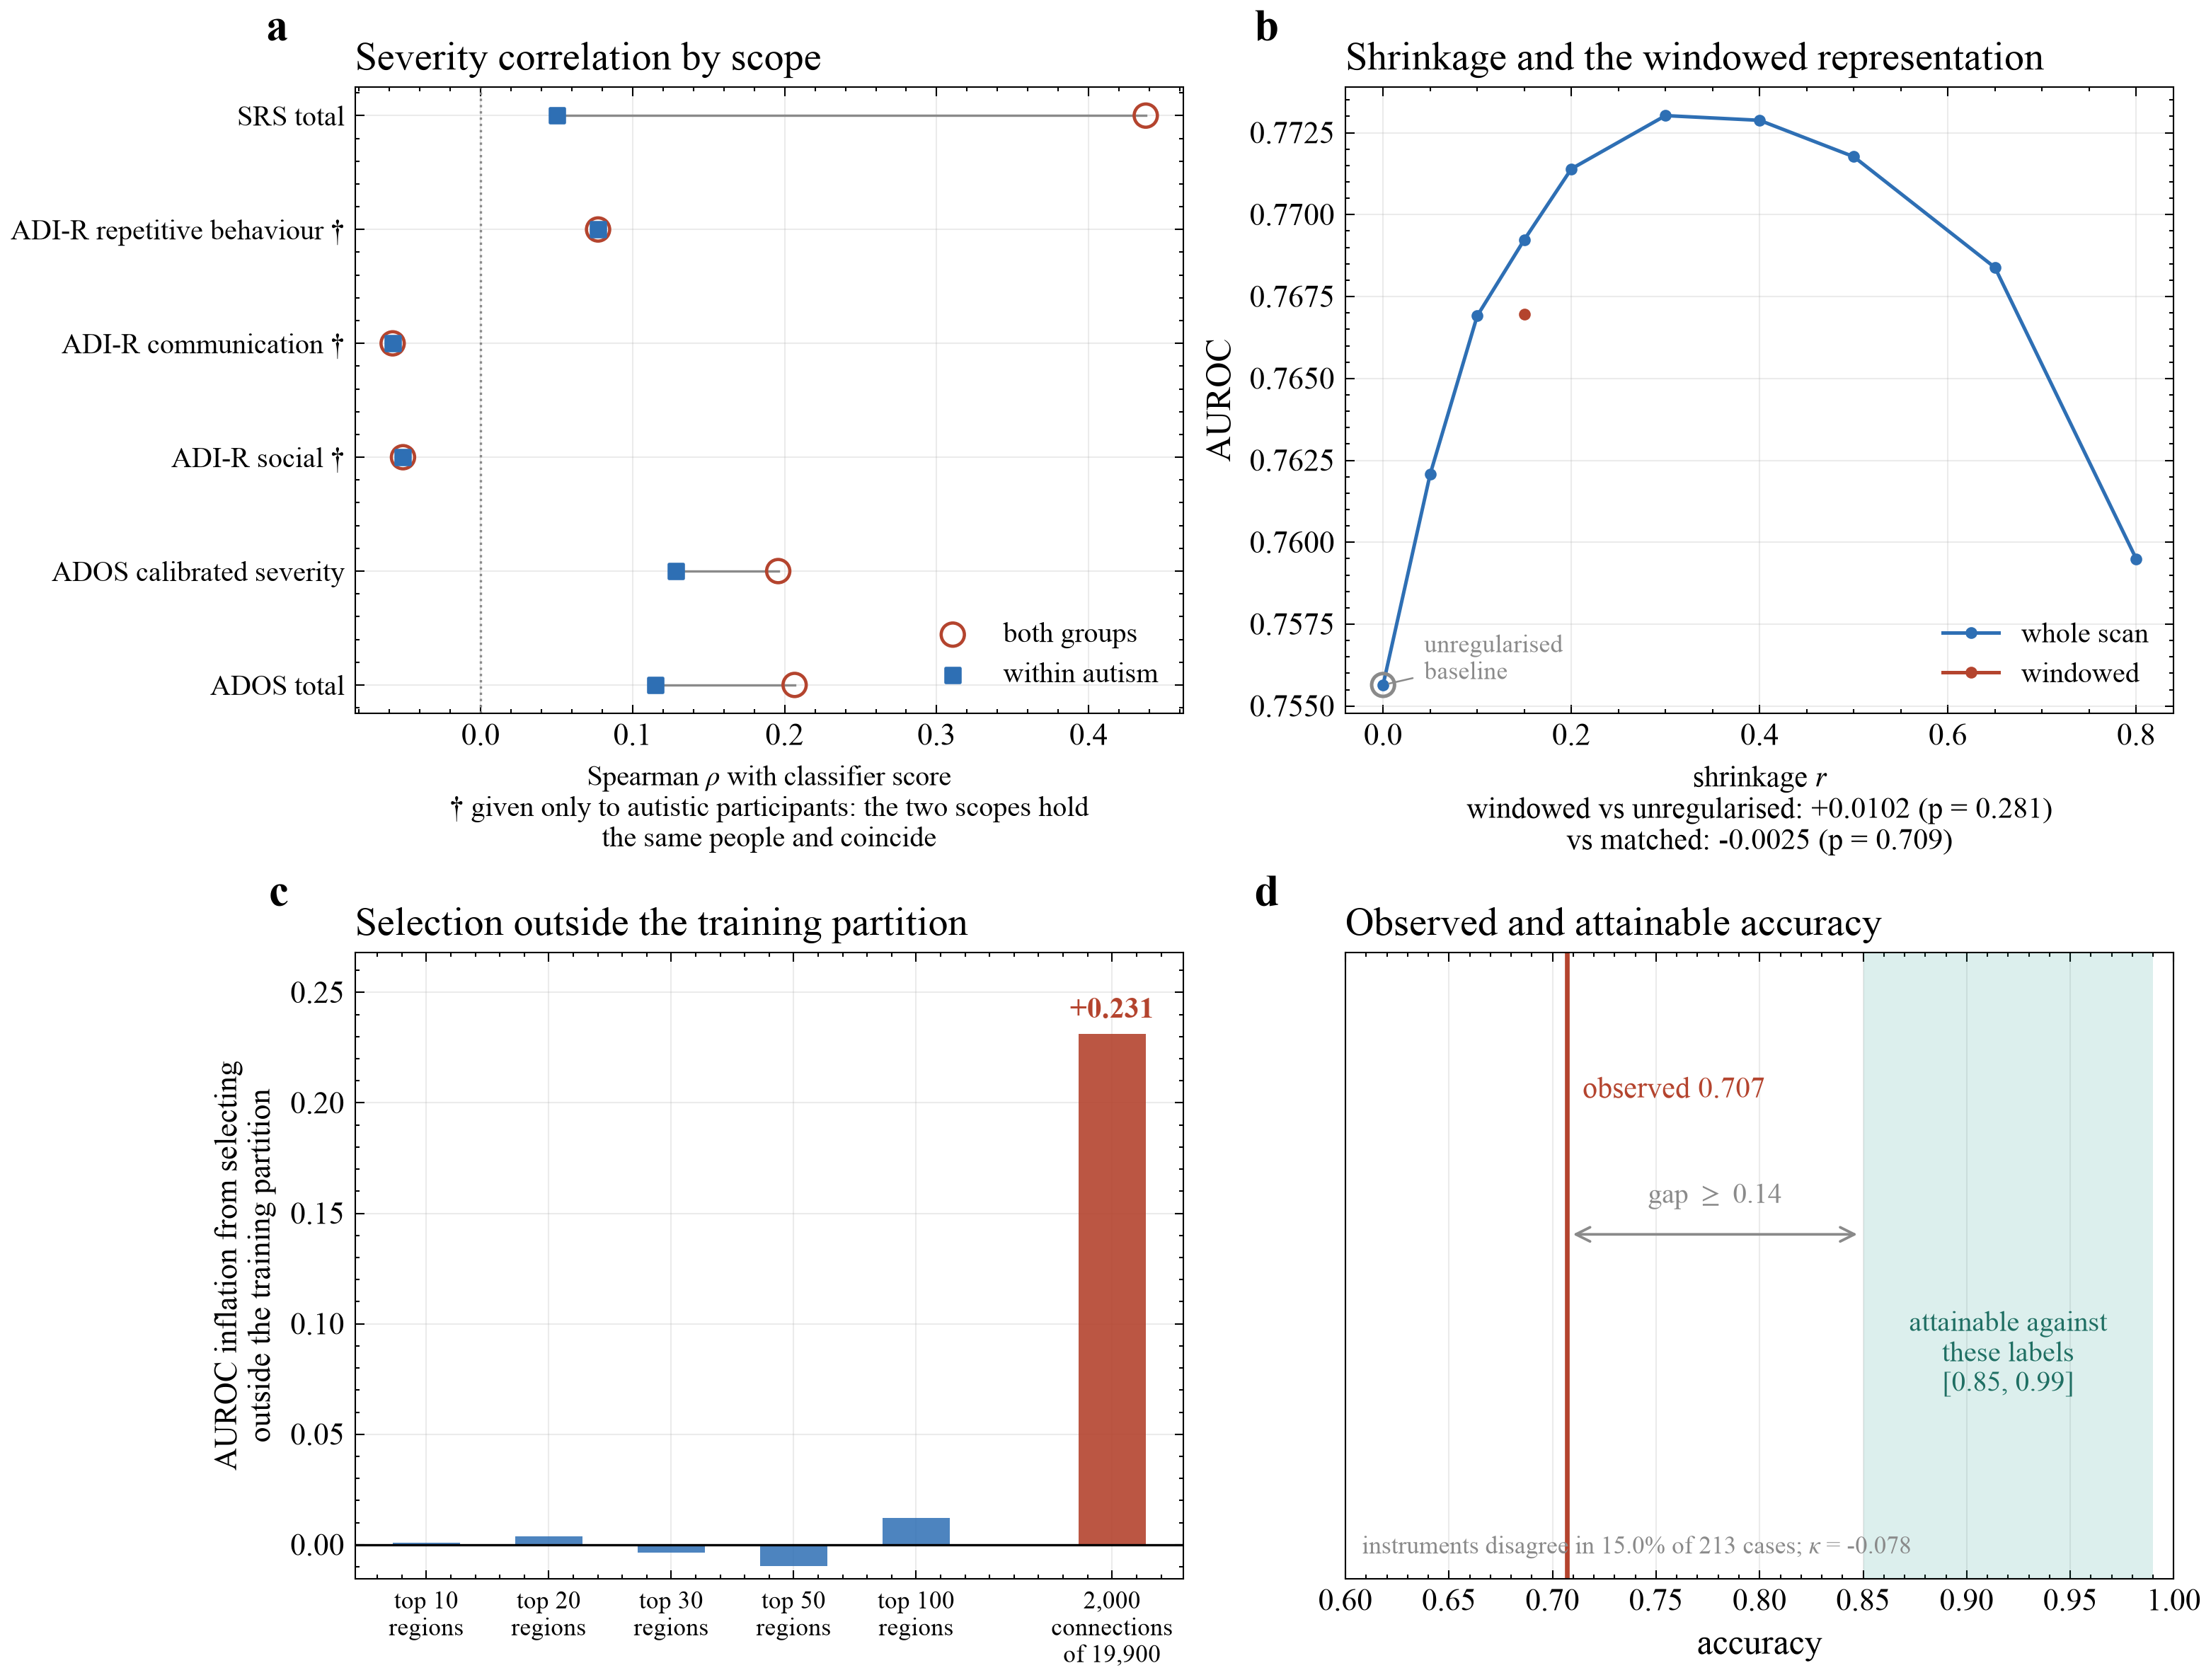
\includegraphics[width=\linewidth]{fig_corrections}
\caption{Four effects that change when the corresponding control is applied. (a)
Correlation between classifier score and symptom severity under pooled ten-fold validation,
computed across both groups and within the autistic group; rows marked with a dagger are
instruments given only to autistic participants, for which the two scopes necessarily coincide.
(b) AUROC of whole-scan connectivity across shrinkage levels, with the windowed
representation placed at the shrinkage that it applies to its own windows. (c) AUROC
inflation from selection outside the training partition, for 10 to 100 of 196 regions and
for 2,000 of 19,900 connections. (d) Observed accuracy against the interval of accuracy
attainable given the diagnostic labels.}
\label{fig:corrections}
\end{figure}

Restricting the model to the most discriminating regions reduces performance at every list length. Using all 196 regions gives an AUROC of 0.781, higher than any reduced set in Table~\ref{tab:region-selection}, while the smallest subset is lower by 0.154. This pattern suggests that discriminative information is distributed across many regions rather than concentrated only in those with the largest group differences. Region restriction therefore provides no performance advantage in these data. More broadly, the published accuracy range is already reached without feature selection before the split. In the wider cohort, the ensemble achieves a participant-pooled accuracy of 0.706 under pooled ten-fold validation (Section~\ref{subsec:results-performance}), compared with published values of 0.700, 0.703, and 0.708 for the same eligible count of 1,035 participants. Accuracy at this level therefore does not require selection outside the training partition.

\subsection{Classifier family}
\label{subsec:results-classifier-family}

Linear classifiers perform better than the evaluated fixed-configuration tree ensembles on static tangent connectivity, forming part of the fifth study contribution. All eight classifiers use the same features, scaling procedure, and outer folds (Section~\ref{par:classifier-family}), so the comparison is made under a common input and validation setting. The five linear classifiers achieve participant-pooled AUROCs of 0.735--0.757, compared with 0.611--0.624 for random forest, XGBoost, and CatBoost (Table~\ref{tab:classifier-family}). Penalised logistic regression gives the highest AUROC at 0.757, followed closely by ridge classification at 0.755 and linear SVC at 0.753. Shrinkage LDA and the rank-20 spectral model achieve AUROCs of 0.741 and 0.735, respectively. Because only logistic regression is tuned, these results compare the specified classifier configurations rather than the best attainable performance of each model family.

\begin{table}[t]
\centering
\caption{Classifier family on the static tangent features of the primary cohort
(871 participants), with identical features, scaling and outer folds. Only logistic
regression is tuned; the other classifiers use fixed configurations.}
\label{tab:classifier-family}
\small
\setlength{\tabcolsep}{4pt}
\begin{tabular}{@{}lcccc@{}}
\toprule
Classifier & AUROC (participant-pooled) & AUROC (fold mean) & SD (folds) & Accuracy (fold mean) \\
\midrule
Logistic regression & 0.757 & 0.756 & 0.048 & 0.692 \\
Ridge & 0.755 & 0.755 & 0.047 & 0.693 \\
Linear SVC & 0.753 & 0.753 & 0.048 & 0.687 \\
Shrinkage LDA (PCA-200) & 0.741 & 0.739 & 0.052 & 0.669 \\
Low-rank spectral (rank 20) & 0.735 & 0.737 & 0.044 & 0.672 \\
CatBoost & 0.624 & 0.623 & 0.042 & 0.597 \\
XGBoost & 0.617 & 0.616 & 0.050 & 0.584 \\
Random forest & 0.611 & 0.609 & 0.049 & 0.577 \\
\bottomrule
\end{tabular}
\end{table}

The performance gap between logistic regression and the tree ensembles is substantial. Logistic regression exceeds XGBoost by 0.1396 AUROC, random forest by 0.1461, and CatBoost by 0.1327, with unadjusted DeLong $p$-values ranging from $6.3\times10^{-15}$ to $2.4\times10^{-12}$ (Section~\ref{subsubsec:paired-comparisons}). By comparison, the rank-20 spectral model is 0.0214 below logistic regression (unadjusted $p=0.0439$; $q=0.1065$, reported for reference only). These results describe the specific configurations evaluated rather than the best possible performance of each classifier family, because only logistic regression is tuned while the tree ensembles use fixed settings (Section~\ref{par:classifier-family}). However, the fixed-configuration ridge, linear SVC, and LDA models also outperform all three tree ensembles. The stronger performance of the linear configurations therefore cannot be explained by logistic-regression tuning alone.

\subsection{Scope of the symptom-severity associations}
\label{subsec:results-symptom-severity}

The symptom analyses show that classifier scores are associated with symptom measures mainly when both diagnostic groups are analysed together, forming part of the fourth study contribution (Figure~\ref{fig:corrections}a). Under pooled ten-fold validation, 3 of 6 associations survive BH-FDR correction across both groups, whereas none survives within autistic participants alone (Section~\ref{par:symptom-associations}). The clearest example is the SRS total, for which the correlation falls from $\rho=0.438$ across both groups ($n=300$) to 0.050 within autistic participants ($n=163$). The corresponding values are 0.207 versus 0.115 for ADOS total and 0.196 versus 0.128 for ADOS calibrated severity. For the ADI-R domains, the correlations are unchanged because these measures are available only for autistic participants. These results indicate that the pooled associations largely reflect diagnostic-group separation, while an association between classifier score and symptom severity within autistic participants is not established.

\subsection{Windowed connectivity and covariance shrinkage}
\label{subsec:results-windowed-shrinkage}

The apparent advantage of windowed connectivity is small and disappears when the whole-scan representation receives the same additional covariance shrinkage, forming part of the fifth study contribution (Figure~\ref{fig:corrections}b). The windowed representation applies an additional shrinkage of 0.15 to its covariance estimates, whereas the original static representation does not (Section~\ref{subsubsec:primary-comparisons}). Applying the same shrinkage to the static representation increases its AUROC by 0.013 (unadjusted DeLong $p=0.004$). By comparison, the windowed representation exceeds the unshrunk static baseline by 0.010 ($p=0.281$) but differs from the shrinkage-matched static baseline by only $-0.002$ ($p=0.709$). Thus, the observed windowed advantage is consistent with the effect of additional covariance shrinkage rather than with added information from windowing itself.

\subsection{Calibration and recalibration within the training partitions}
\label{subsec:results-calibration}

The native ensemble probabilities show calibration slopes close to one but a small systematic offset in their average predicted risk, and training-partition recalibration removes this offset without changing discrimination; this forms the first study contribution (Table~\ref{tab:calibration-recalibration}; Figure~\ref{fig:calibration}). Under pooled ten-fold validation, the native calibration slope is 1.117 (95\% site-clustered bootstrap interval 0.901--1.325), and under LOSO validation it is 1.120 (0.866--1.366), with both intervals including one. Calibration-in-the-large is $-0.162$ ($-0.287$ to $-0.048$) under pooled validation and $-0.181$ ($-0.389$ to 0.019) under LOSO validation, indicating that the native probabilities tend to overestimate autism prevalence on average. The Brier score is 0.194 under both protocols, corresponding to Brier skill scores of 0.221 and 0.218 relative to a prevalence-only model. ECE varies with the binning choice: under pooled validation it is 0.037 with five bins, 0.046 with ten, and 0.059 with twenty, while the smallest bins contain 86, 17, and 0 participants, respectively. ECE is therefore reported together with the number of bins rather than as a single standalone calibration measure (Figure~\ref{fig:calibration}a,b).

\begin{table}[t]
\centering
\caption{Ensemble probabilities are evaluated before and after recalibration fitted within each outer training partition. Calibration-in-the-large, where negative values indicate over-prediction of autism, and the calibration slope are reported with 95\% site-clustered bootstrap intervals. ECE is calculated using ten equal-width bins, and accuracy is measured at a threshold of 0.5. The final row of each block is included as a diagnostic, with the ensemble members refitted using an unpenalised intercept.}
\label{tab:calibration-recalibration}
\footnotesize
\setlength{\tabcolsep}{3pt}
\begin{tabular}{@{}lcccccc@{}}
\toprule
Correction & Calibration-in-the-large & Slope & Brier & ECE & AUROC & Accuracy \\
\midrule
\multicolumn{7}{@{}l}{\textit{Pooled ten-fold validation}} \\
Native & $-0.162$ ($-0.287$ to $-0.048$) & 1.117 (0.901 to 1.325) & 0.194 & 0.046 & 0.776 & 0.707 \\
Intercept (primary) & $-0.010$ ($-0.136$ to 0.103) & 1.115 (0.898 to 1.324) & 0.193 & 0.040 & 0.776 & 0.713 \\
Logistic & $-0.010$ ($-0.143$ to 0.105) & 1.026 (0.824 to 1.218) & 0.192 & 0.037 & 0.776 & 0.711 \\
Isotonic & 0.000 ($-0.139$ to 0.117) & 0.855 (0.654 to 1.043) & 0.194 & 0.018 & 0.771 & 0.707 \\
Unpenalised intercept (diagnostic) & $+0.061$ ($-0.066$ to 0.175) & 1.114 (0.902 to 1.316) & 0.193 & 0.044 & 0.776 & 0.720 \\
\midrule
\multicolumn{7}{@{}l}{\textit{LOSO validation}} \\
Native & $-0.181$ ($-0.389$ to 0.019) & 1.120 (0.866 to 1.366) & 0.194 & 0.040 & 0.774 & 0.711 \\
Intercept (primary) & $+0.023$ ($-0.186$ to 0.235) & 1.115 (0.860 to 1.366) & 0.194 & 0.027 & 0.774 & 0.701 \\
Logistic & $+0.012$ ($-0.189$ to 0.227) & 1.159 (0.899 to 1.493) & 0.195 & 0.033 & 0.769 & 0.705 \\
Isotonic & $-0.006$ ($-0.214$ to 0.228) & 0.989 (0.733 to 1.284) & 0.197 & 0.021 & 0.766 & 0.698 \\
Unpenalised intercept (diagnostic) & $+0.036$ ($-0.180$ to 0.256) & 1.105 (0.857 to 1.353) & 0.194 & 0.030 & 0.772 & 0.705 \\
\bottomrule
\end{tabular}
\end{table}



\begin{figure}[pos=tbp]
\centering
\includegraphics[width=\linewidth]{fig_calibration}
\caption{Calibration of the ensemble probabilities. (a) Reliability under pooled ten-fold validation and (b) reliability under LOSO validation, using ten equal-width bins with Wilson intervals for the observed proportion and marker area proportional to the number of participants per bin. Native probabilities are shown with intercept and logistic corrections fitted within the training partitions. (c) Calibration-in-the-large with 95\% site-clustered bootstrap intervals; pooled validation is shown in the upper block and LOSO validation in the lower block, with the unpenalised-intercept refit included as a diagnostic. (d) Site-level calibration-in-the-large for withheld sites with at least 30 participants, shown before and after intercept correction, with Wald intervals for the native probabilities.}
\label{fig:calibration}
\end{figure}


The calibration offset appears to arise mainly from intercept penalisation in the original solver. Because the intercept is penalised together with the feature weights, it is drawn towards zero, shifting the predicted probability of an average participant towards 0.5 even though the autistic proportion in the training partitions is 0.463. Consistent with this mechanism, the mean fitted intercept is $-0.017$. Refitting the ensemble members with an unpenalised intercept moves the mean intercept to $-0.253$ and shifts calibration-in-the-large from $-0.162$ to $+0.061$ ($-0.066$ to 0.175) under pooled validation and from $-0.181$ to $+0.036$ ($-0.180$ to 0.256) under LOSO validation. This refit is used only as a diagnostic. The primary intercept-only recalibration, fitted within each outer training partition, reduces calibration-in-the-large to $-0.010$ ($-0.136$ to 0.103) under pooled validation and $+0.023$ ($-0.186$ to 0.235) under LOSO validation (Table~\ref{tab:calibration-recalibration}). The learned logit shift is also stable across pooled outer folds, ranging from $-0.172$ to $-0.138$. Discrimination is essentially unchanged, with AUROC differences of $-0.0001$ ($-0.0005$ to 0.0004) and $-0.0010$ ($-0.0026$ to 0.0007) under the two protocols. Changes in Brier score, calibration slope, and ECE are likewise small and not clearly separated from sampling variation. More flexible recalibration provides no consistent advantage. Logistic recalibration gives a slope of 1.026 under pooled validation but 1.159 under LOSO validation, while changes in Brier score remain small. Isotonic recalibration lowers the ten-bin ECE to 0.018 and 0.021, but AUROC decreases by $-0.0048$ and $-0.0083$, with the LOSO interval excluding zero ($-0.0137$ to $-0.0004$). The primary recalibration also changes threshold-based decisions at 0.5. Under pooled validation, sensitivity falls from 0.705 to 0.655 while specificity rises from 0.709 to 0.763, with little change in accuracy ($+0.006$, $-0.011$ to 0.024). Under LOSO validation, sensitivity falls from 0.742 to 0.625, specificity rises from 0.684 to 0.767, and accuracy changes from 0.711 to 0.701 ($-0.009$, $-0.029$ to 0.017). Thus, recalibration preserves ranking but shifts the operating point towards greater specificity at the fixed threshold. Site-level calibration remains more variable. Among the 10 sites with at least 30 participants, pooled validation shows little residual heterogeneity after recalibration ($Q=6.4$ on 9 degrees of freedom, $I^2=0\%$), whereas LOSO validation retains substantial heterogeneity ($Q=24.1$ on 9 degrees of freedom, $I^2=63\%$, between-site SD 0.37). Before recalibration, KKI and TRINITY have intervals excluding zero; afterwards, KKI and USM do so. These site-level differences are consistent with variation in site-specific outcome prevalence, as KKI and USM have the lowest and highest autistic proportions among these sites (0.36 and 0.64). Overall, the intercept-only correction removes the average calibration offset without changing discrimination, but it does not eliminate calibration differences across sites.

\subsection{Attribution of the score to functional-system pairs}
\label{subsec:results-interpretation}

The ensemble score is attributed exactly to the 36 functional-system pairs, and this attribution forms the second contribution of the study (Table~\ref{tab:system-contributions}; Figure~\ref{fig:interpretation}). Reproducibility is observed at the system-pair level, with weaker reproducibility found for individual connections. Each held-out score is reproduced by the summed pair contributions within $10^{-14}$, and the stored probabilities are reproduced by the stored weights within $10^{-7}$. Averaged across the three views, between-group separation is estimated at 1.07 logit units under pooled validation and 1.06 when a site is withheld. Zero is excluded from the contribution-difference intervals for 28 of the 37 connection groups under pooled validation and for 28 groups under site-held-out validation, with no negative contribution difference observed (Figure~\ref{fig:interpretation}a). The separation is therefore distributed across many functional-system pairs rather than being concentrated in a small number of pairs.

\begin{table}[t]
\centering
\caption{System pairs carrying the largest share of separation between autistic and non-autistic participants are identified from held-out scores averaged across the three ensemble views. The share is calculated as the between-group difference in mean contribution divided by the total difference in mean score, with 95\% site-clustered bootstrap intervals reported on the same scale. AUROC is calculated from each pair's contribution alone. Familywise $p$-values are obtained by comparing each AUROC with the maximum deviation from 0.5 across all 36 pairs under within-site label permutation. The total difference in mean score is 1.069 on the logit scale, of which 5.7\% is carried by connections involving the four regions excluded from the group-difference analyses.}
\label{tab:system-contributions}
\footnotesize
\setlength{\tabcolsep}{3pt}
\begin{tabular}{@{}llcccc@{}}
\toprule
System & System & Connections & Share (\%) & AUROC & Familywise $p$ \\
\midrule
Default mode & Default mode & 903 & 12.9 (9.6 to 15.5) & 0.690 (0.646 to 0.727) & 0.010 \\
Default mode & Subcortical / cerebellar & 1{,}462 & 9.4 (6.2 to 12.0) & 0.627 (0.587 to 0.659) & 0.010 \\
Visual & Default mode & 1{,}290 & 6.4 (3.6 to 8.6) & 0.632 (0.574 to 0.678) & 0.010 \\
Frontoparietal control & Default mode & 903 & 5.7 (2.8 to 8.1) & 0.607 (0.552 to 0.652) & 0.010 \\
Somatomotor & Default mode & 903 & 4.4 (2.9 to 6.4) & 0.596 (0.567 to 0.636) & 0.030 \\
Salience / ventral attention & Default mode & 903 & 3.9 (2.0 to 5.5) & 0.599 (0.548 to 0.639) & 0.020 \\
Visual & Salience / ventral attention & 630 & 3.8 (2.4 to 5.0) & 0.616 (0.573 to 0.655) & 0.010 \\
Somatomotor & Somatomotor & 210 & 3.7 (2.3 to 5.0) & 0.589 (0.556 to 0.624) & 0.079 \\
Visual & Dorsal attention & 570 & 3.3 (2.2 to 4.4) & 0.600 (0.561 to 0.639) & 0.020 \\
Visual & Visual & 435 & 3.2 (1.6 to 4.9) & 0.574 (0.536 to 0.610) & 0.386 \\
\bottomrule
\end{tabular}
\end{table}


\begin{figure}[pos=tbp]
\centering
\includegraphics[width=\linewidth]{fig_interpretation}
\caption{Attribution of the ensemble score to functional-system pairs (system codes as in Figure~\ref{fig:overview}). (a) Between-group difference in mean contribution per connection, averaged across the three views and pooled held-out predictions; asterisks mark pairs whose held-out AUROC exceeds the permutation maximum (familywise $p<0.05$). (b) Held-out AUROC for each pair alone, with 95\% site-clustered bootstrap intervals; filled markers indicate familywise $p<0.05$. (c) Spearman correlation of structure coefficients between independent cohort halves for each view and level; black ticks show the 95th percentile under diagnosis permutation. (d) Held-out AUROC after the highest-ranked system pairs from the training fit are deleted or retained alone, compared with random pairs; the dashed line and shading show the random-pair mean and 95\% range.}
\label{fig:interpretation}
\end{figure}


System-pair contributions show that default mode connections account for the largest shares of model separation. The within-default-mode contribution explains 12.9\% of the separation (interval 9.6--15.5), followed by default mode--subcortical/cerebellar at 9.4\% and visual--default mode at 6.4\% (Table~\ref{tab:system-contributions}). Because these shares depend partly on pair size (Spearman $\rho=0.72$ with the number of connections), contributions are also examined per connection. On this scale, the largest effect occurs within the somatomotor system (0.187$\times10^{-3}$ logit), followed by within-default-mode (0.153$\times10^{-3}$) and visual--limbic connectivity (0.143$\times10^{-3}$), consistent with the strongest univariate system differences in Table~\ref{tab:system-pairs}. Connections involving the four regions excluded from the group-difference analysis account for 5.7\% of the separation and are interpreted cautiously because these regions contain constant signals in some participants. Individual system pairs provide only moderate discrimination on held-out participants: the within-default-mode contribution reaches an AUROC of 0.690 (0.646--0.727), and 13 of 36 pairs exceed the familywise permutation reference. Across the correlation, static tangent, and windowed views, 5, 10, and 9 pairs, respectively, exceed this reference (Figure~\ref{fig:interpretation}b); pairs that do not exceed it are not interpreted as having no signal. Apparent agreement across overlapping training partitions is high, with structure-coefficient correlations of 0.91--0.96, but similar agreement is also observed after label permutation, confirming that overlap between training sets inflates this measure. Reproducibility is therefore assessed using independent split halves (Table~\ref{tab:pattern-reproducibility}; Figure~\ref{fig:interpretation}c). At the system-pair level, structure coefficients correlate at 0.60, 0.70, and 0.68 across halves for the correlation, static tangent, and windowed views, exceeding permutation 95th percentiles of 0.08, 0.12, and 0.13. The corresponding correlations are 0.35, 0.24, and 0.30 at the regional level and 0.53, 0.18, and 0.30 at the connection level. System-pair signs agree in 64\%, 78\%, and 71\% of cases, compared with 51\%--55\% under permutation. Thus, system-level patterns show the strongest reproducibility across independent halves, while individual tangent-space connections are less stable. Classifier weights are also less reproducible than structure coefficients, with system-pair correlations of 0.33, 0.55, and 0.44.

\begin{table}[t]
\centering

\caption{Agreement between patterns fitted in two independent halves of the cohort, reported as the mean Spearman correlation across 40 random splits. For each connection, the structure coefficient is its correlation with the model score, and the weight is its model coefficient. Values in brackets show the 95th percentile obtained after within-site diagnosis permutation. Sign agreement is the percentage of connections, regions, or system pairs with the same structure-coefficient sign in both halves, with the permutation mean shown in brackets.}

\label{tab:pattern-reproducibility}
\small
\begin{tabular}{@{}llccc@{}}
\toprule
View & Level & Structure coefficients $\rho$ & Sign agreement (\%) & Weights $\rho$ \\
\midrule
Correlation & Connections & 0.530 (0.045) & 64 (51) & 0.152 (0.008) \\
 & Regions & 0.346 (0.044) & 47 (51) & 0.149 (0.024) \\
 & System pairs & 0.603 (0.080) & 64 (51) & 0.334 (0.049) \\
\midrule
Static tangent & Connections & 0.179 (0.015) & 56 (50) & 0.092 (0.005) \\
 & Regions & 0.240 (0.067) & 54 (53) & 0.128 (0.029) \\
 & System pairs & 0.701 (0.118) & 78 (55) & 0.547 (0.078) \\
\midrule
Windowed tangent, mean & Connections & 0.302 (0.028) & 60 (51) & 0.128 (0.006) \\
 & Regions & 0.301 (0.072) & 58 (53) & 0.141 (0.029) \\
 & System pairs & 0.676 (0.126) & 71 (55) & 0.442 (0.079) \\
\bottomrule
\end{tabular}
\end{table}


The three connectivity views show different levels of agreement. Static tangent and windowed connectivity are highly similar across the 36 system pairs (Spearman correlation 0.90), whereas the correlation view agrees less strongly with the static tangent and windowed views (0.55 and 0.64). The correlation view also aligns closely with the nuisance-adjusted system-level group differences, with correlations of 0.93 in the full cohort and 0.89 after motion matching. The corresponding values are lower for static tangent connectivity (0.43 and 0.58) and windowed connectivity (0.55 and 0.73). Within the somatomotor system, regional patterns agree strongly with the regional group differences in all three views (0.93, 0.79, and 0.78). Because the classifier itself is not adjusted for site, motion, age, or sex, this agreement is interpreted as descriptive rather than as a direct validation of the classifier. The highest-ranked system pairs also contribute meaningfully to held-out predictions (Figure~\ref{fig:interpretation}d). Removing the 12 highest-ranked pairs reduces AUROC from 0.776 to 0.707, compared with 0.757 for 12 randomly selected pairs (95\% range 0.743--0.771). Conversely, retaining only the 3 highest-ranked pairs, together with the unassigned connections, gives an AUROC of 0.763, compared with 0.655 for 3 random pairs. Similar patterns are observed under LOSO validation: AUROC falls to 0.710 after removing the highest-ranked pairs, compared with 0.756 for random removal, while retaining the highest-ranked pairs gives 0.749 compared with 0.648 for random retention. Because these analyses remove or retain features without refitting the model, they show which system pairs the trained classifier relies on rather than whether a newly fitted model could compensate for their absence. The information is nevertheless distributed across multiple pairs, as removing the 6 highest-ranked pairs lowers AUROC by only 0.037.

\subsection{Secondary results}
\label{subsec:results-secondary}

The remaining analyses are reported as descriptive results and are not treated as study contributions. The first examines confidence-based abstention using ensemble probabilities after calibration assessment (Section~\ref{subsec:results-calibration}). In this analysis, abstention does not provide the intended error guarantee for the cases on which the model makes a prediction (Figure~\ref{fig:performance}d; Figure~\ref{fig:abstention-guarantee}). To evaluate the nominal bound, LOSO predictions are randomly divided into two halves, with the confidence threshold selected on one half and evaluated on the other (Section~\ref{subsubsec:threshold-analysis}). This separation avoids evaluating the threshold on the same participants used to select it. When the cohort-wide threshold is selected using the full sample, no participants satisfy the answering criterion. In the half-split analysis, the target error bound is satisfied in 0.8158 of the 38 splits with a finite selective risk, below the nominal level of 0.90. Thus, the abstention procedure does not provide the intended empirical guarantee in this cohort.

\begin{figure}[pos=tbp]
\centering
\includegraphics[width=\linewidth]{fig_guarantee}
\caption{The nominal error bound of the abstention rules under LOSO validation and its evaluation on held-out participants. (a) The error bound that each rule reports on the participants used to set it, against the error that the same rules incur on held-out cases. (b) The cost of each rule for obtaining that bound: the proportion of cases it answers, and the proportion of held-out splits in which it meets its target.}
\label{fig:abstention-guarantee}
\end{figure}

The per-site abstention threshold meets the nominal target, but only at low coverage. When fitted on the full sample, it answers 170 of 871 participants (19.5\%), with 143 of these from a single site and no participants answered at 17 of 20 sites. Across held-out half-splits, mean coverage is 13.7\%, and the target is met in 0.9137 of 197 valid splits. The abstention result is therefore reported as a property of these data rather than as a reliable model feature. Combining multiple atlases also provides no improvement in discrimination. CC200 alone gives a fold-mean AUROC of 0.756, compared with 0.749 when combined with the anatomical labelling atlas, 0.755 with the Harvard--Oxford atlas, and 0.752 with all three (Section~\ref{par:atlas-fusion}). The anatomical atlases perform lower on their own, at 0.692 and 0.717, indicating that the added atlases contribute little beyond CC200. A separate analysis examines how uncertainty in the diagnostic labels may limit attainable accuracy (Figure~\ref{fig:corrections}d). Among 213 autistic participants with complete ADI-R and ADOS information, the instruments disagree in 15.0\% of cases: 13 meet criteria on the interview only, 19 on the observation only, and 181 on both, with none negative on both instruments. Under the assumptions in Section~\ref{par:instrument-concordance}, this corresponds to an illustrative attainable-accuracy range of approximately 0.85--0.99, while the observed accuracy remains about 0.14 below its lower bound. At the central noise rates defined in that section, the correction \citep{Menonetal2015} increases accuracy from 0.707 to 0.729 and AUROC from 0.776 to 0.806. Label uncertainty alone therefore does not account for the observed performance gap under these assumptions. However, the correction becomes larger under more pessimistic noise rates, and the data do not identify the true error rates. Cohen's $\kappa$ is slightly negative ($-0.078$), no participant is negative on both instruments, and the assumptions of the two-rater noise model are not fully supported. For these reasons, the analysis is treated as a sensitivity assessment rather than as a definitive estimate of the performance ceiling.
